\documentclass[journal]{IEEEtran}
%\documentclass[11pt,twoside,a4paper]{article}

\usepackage{url}
\usepackage{amsmath}
\usepackage{amsfonts}
\usepackage{graphicx}
\usepackage[utf8]{inputenc}
\usepackage{subcaption}

%\usepackage[swedish]{babel}
\usepackage[backend=bibtex, citestyle=ieee, bibstyle=ieee]{biblatex}
\addbibresource{ref.bib}

% correct bad hyphenation here
\hyphenation{op-tical net-works semi-conduc-tor}

\begin{document}

\title{Homework 1 \\Critical Sections, Locks, Barriers and Conditional Variables }

\author{Hannes~Rabo, \textit{Information and Communication Technology}, KTH}


% The paper headers
\markboth{Homework 1 - Concurrent Programming (ID1217) - KTH}%
{}

% make the title area
\maketitle


% Note that keywords are not normally used for peerreview papers.
%\begin{IEEEkeywords}
% IEEE, IEEEtran, journal, \LaTeX, paper, template.
%\end{IEEEkeywords}

\IEEEPARstart{IN}{} this homework we study performance of different approaches to concurrent computation. It focuses on matrix operations (sum, min and max) as well as approximation for PI.

\onecolumn
\section{Comparison for Matrix Operations}

\begin{figure}[h]
	\centering
	\begin{subfigure}{0.48\textwidth}
		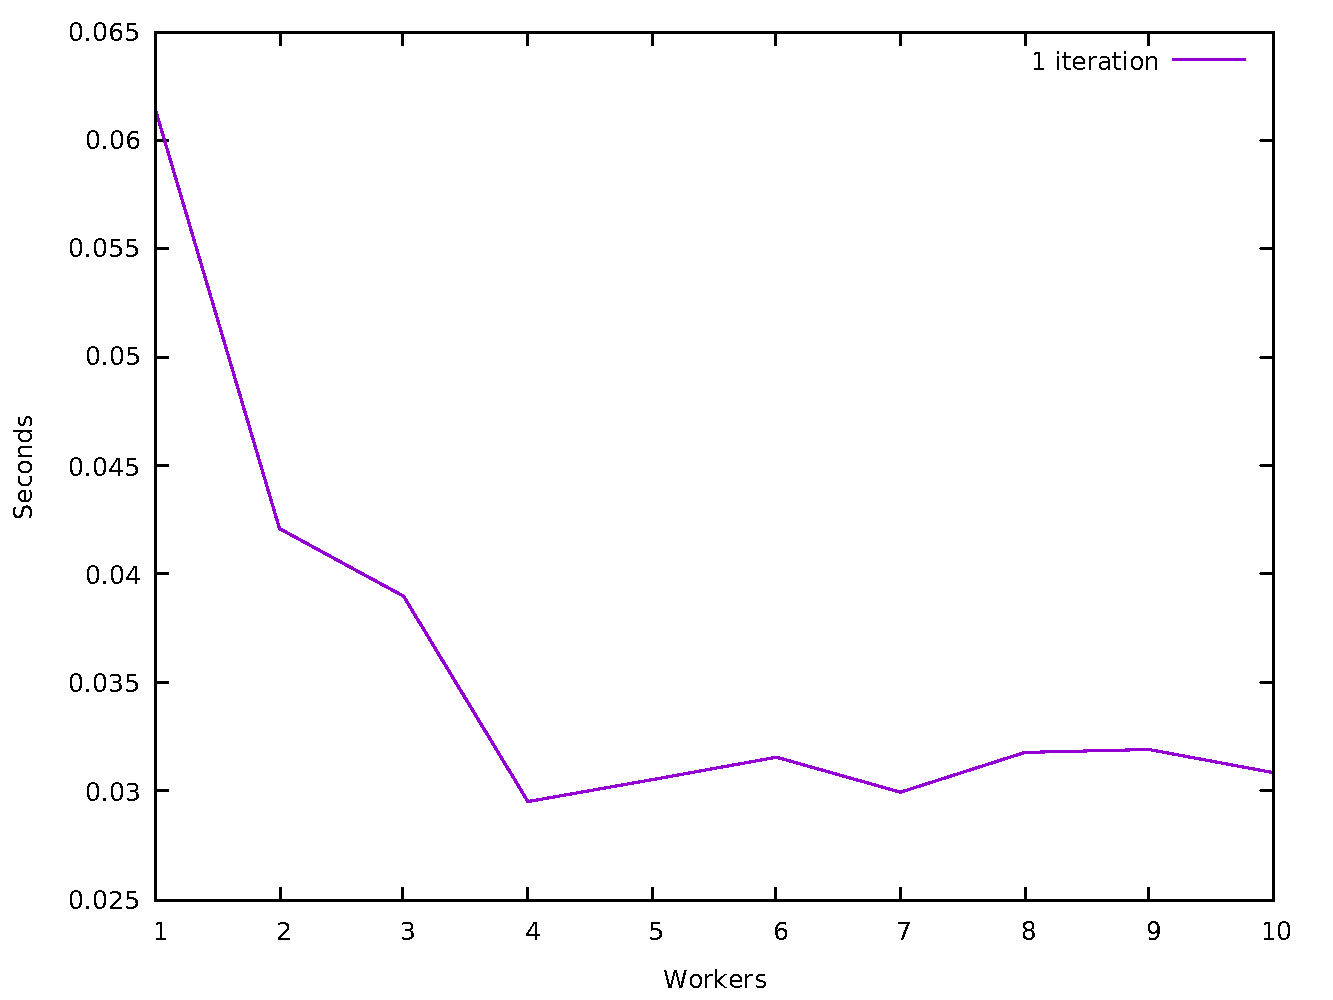
\includegraphics[width=\textwidth]{../results/v1}
		\caption{Version 1: Divide the area in slices. The first thread awaits all others and calculates the total after.}
		\label{fig:v1}
	\end{subfigure}
	~
	\begin{subfigure}{0.48\textwidth}
		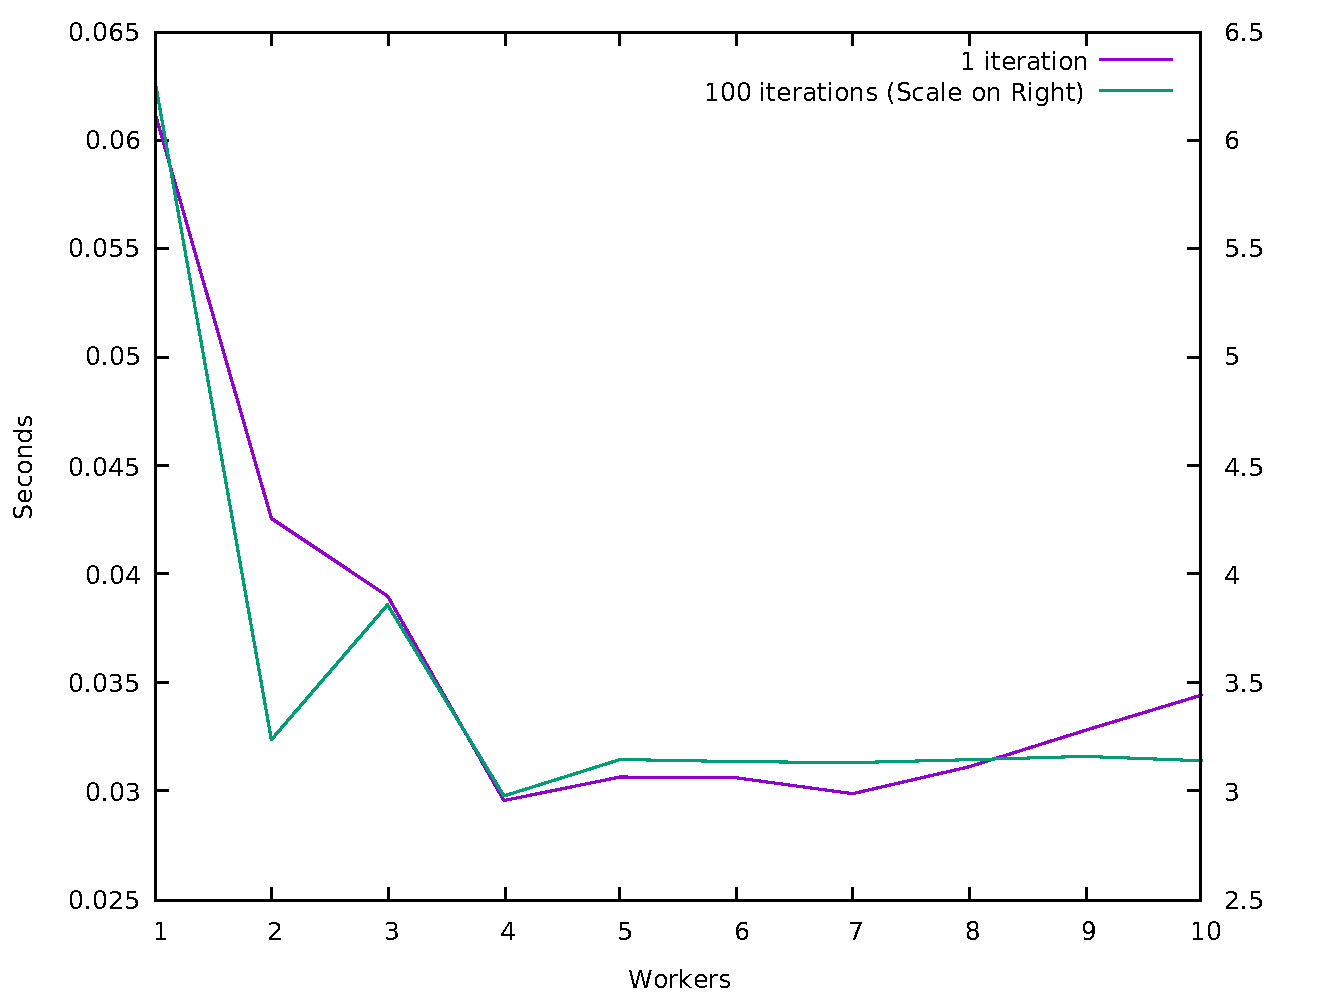
\includegraphics[width=\textwidth]{../results/v2}
		\caption{Version 2: Same approach as a) but total is calculated in main thread. Results are passed as return values and captured by using pthread\_join.}
		\label{fig:v2}
	\end{subfigure}
	\\
	\begin{subfigure}{0.48\textwidth}
		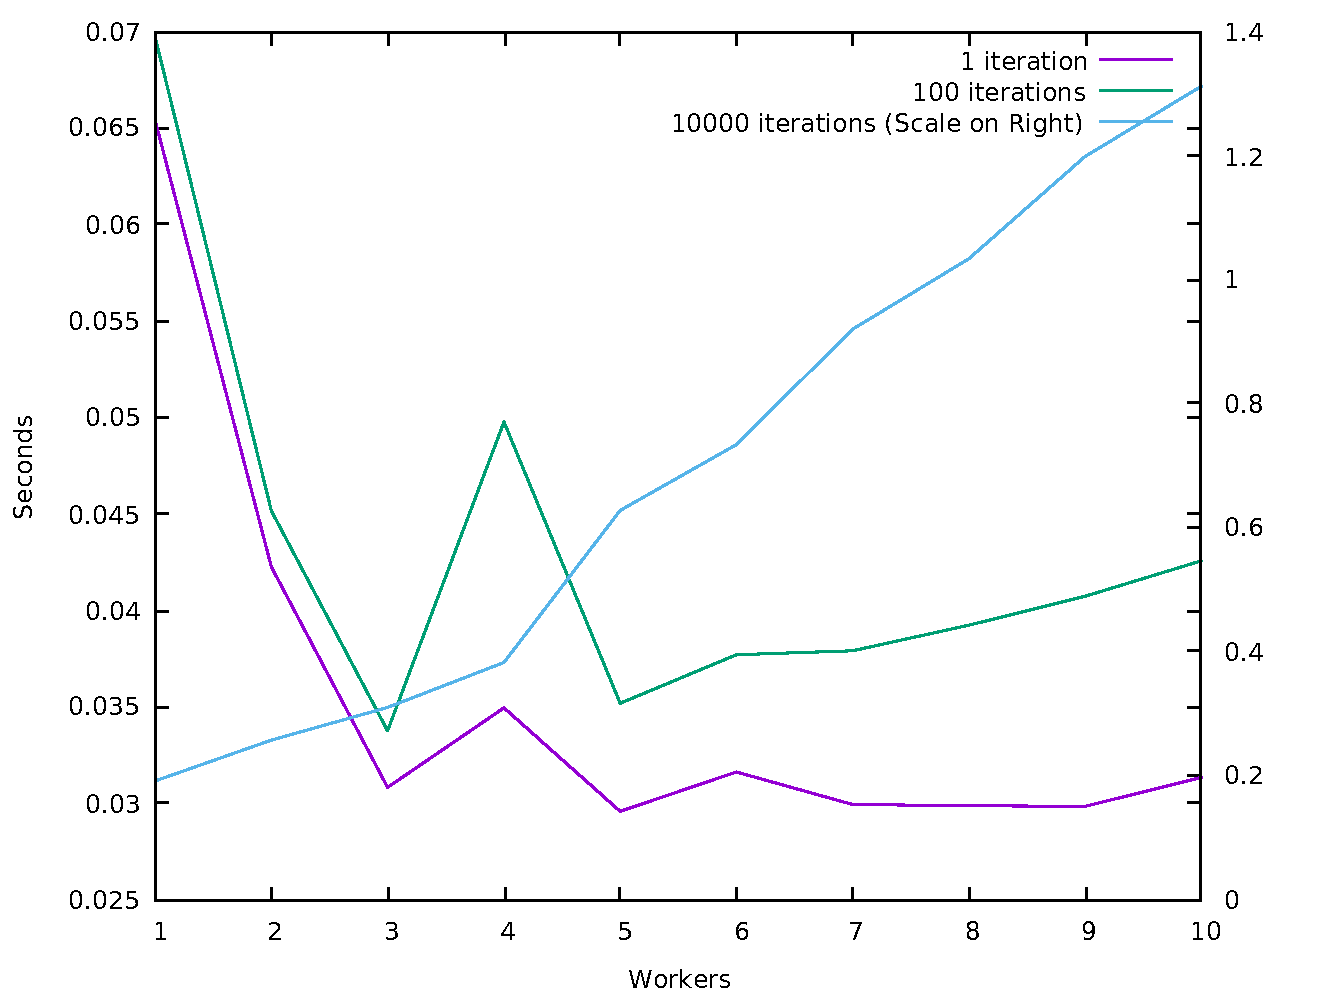
\includegraphics[width=\textwidth]{../results/v3}
		\caption{Version 3: Using workers to calculate matrix operations per row. Main thread calculates result when calculations are complete.}
		\label{fig:v3}
	\end{subfigure}
	~
	\begin{subfigure}{0.48\textwidth}
		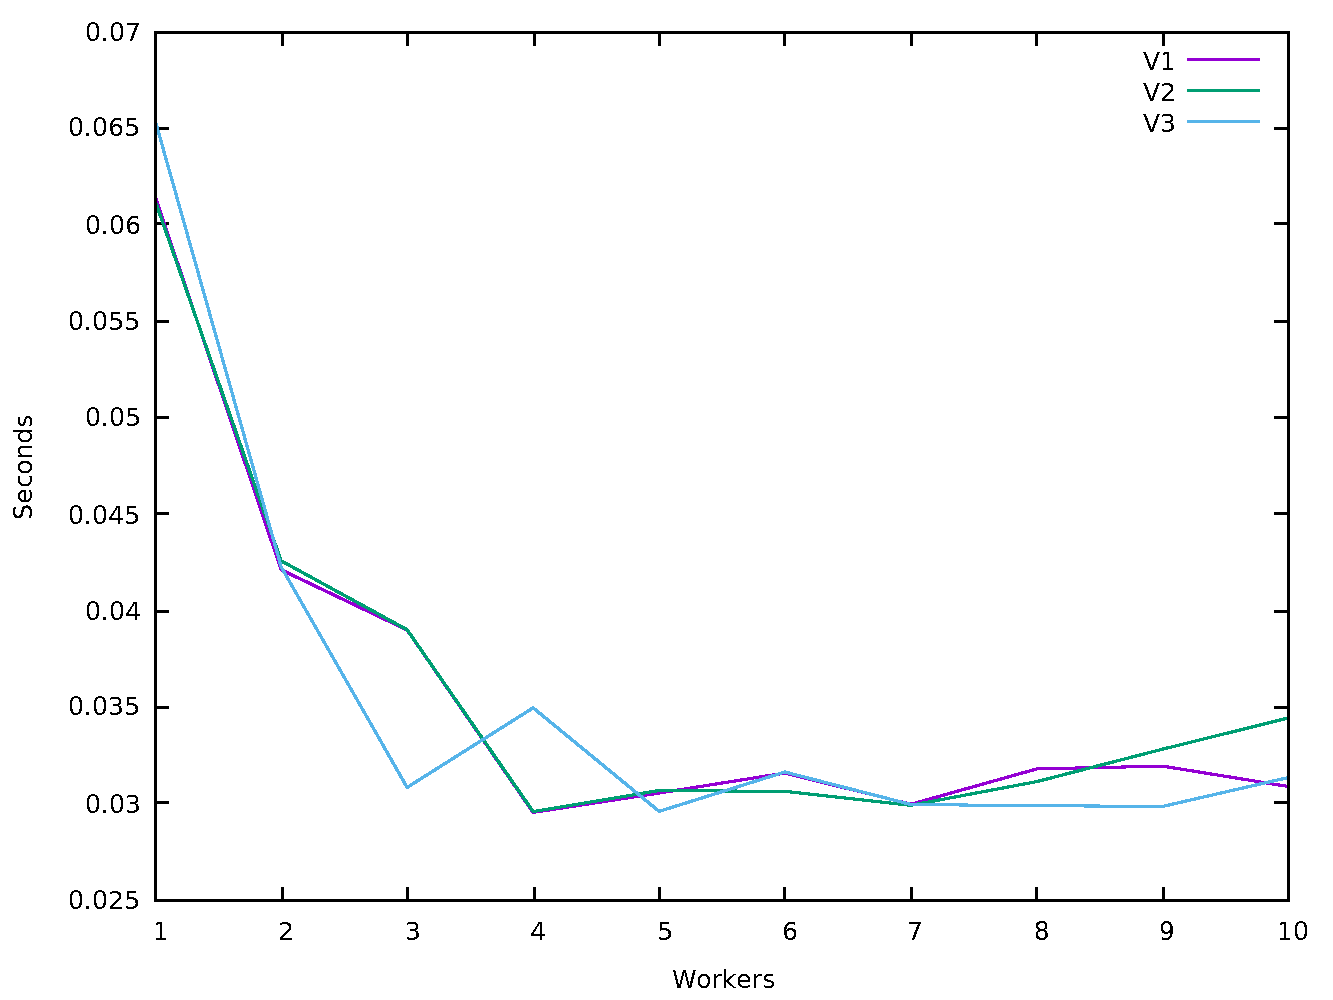
\includegraphics[width=\textwidth]{../results/cmp}
		\caption{Comparison between the different versions}
		\label{fig:cmp}
	\end{subfigure}
	\caption{Comparison between the different parallel matrix operations for matrix size of 10 000 x 10 000}
\end{figure}

\newpage

\section{Approximating Pi}
\begin{figure}[h]
	\centering
	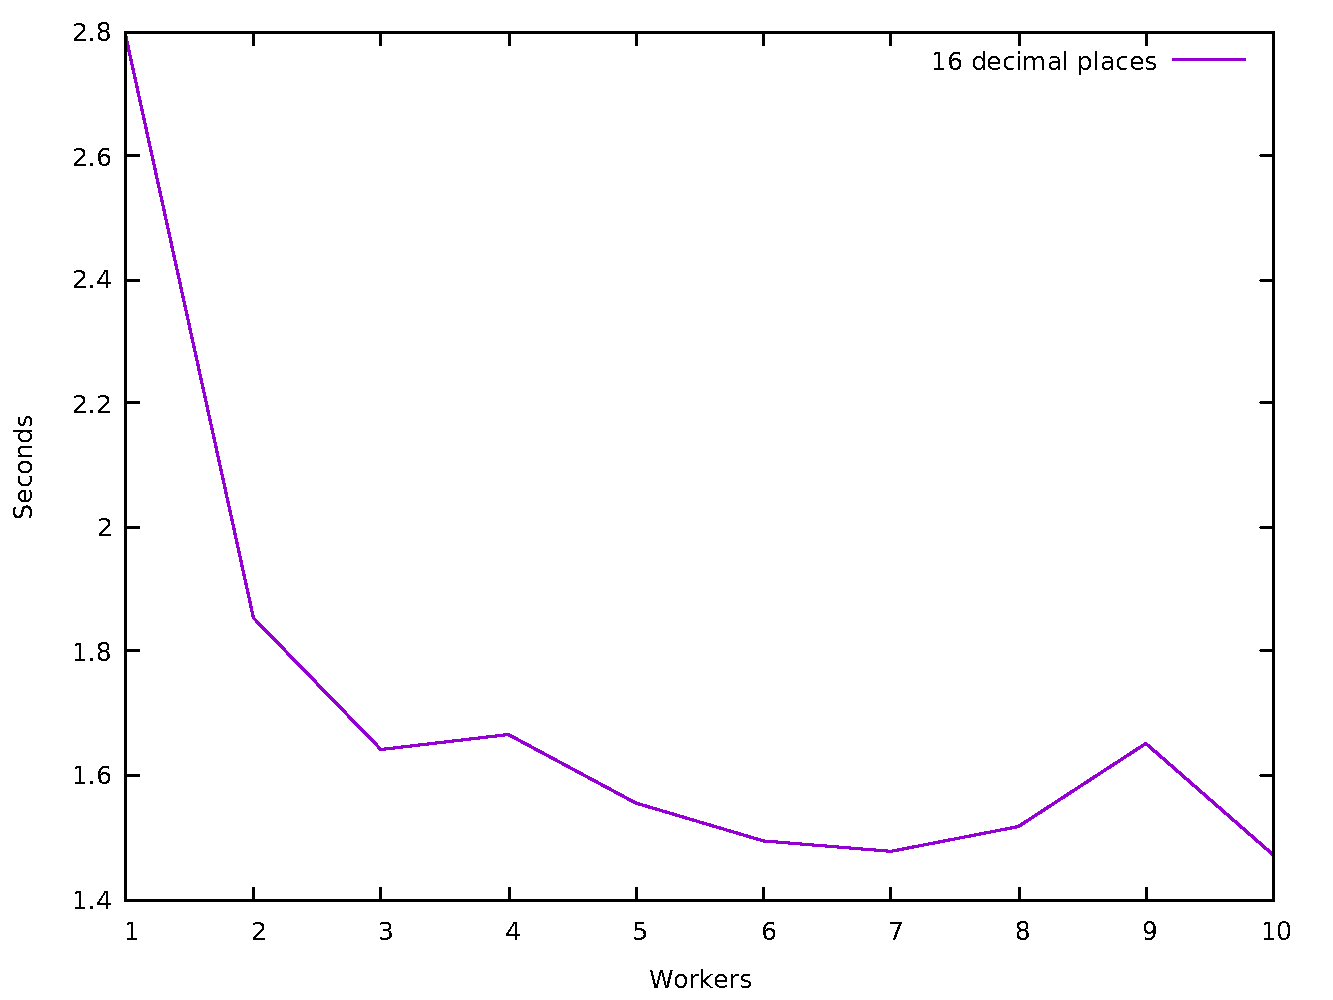
\includegraphics[width=0.7\linewidth]{../results/pi}
	\caption{Performance when calculating pi to 16 decimal places.}
	\label{fig:pi}
\end{figure}



\printbibliography

%\appendices
%\section{Proof of the First Zonklar Equation}
%Appendix one text goes here.
%
%% you can choose not to have a title for an appendix
%% if you want by leaving the argument blank
%\section{}
%Appendix two text goes here.
%

\end{document}


